\chapter{Team 2 Agent Design}
\section{Overall Agent Strategy}

The overall strategy of our agent is based on a series of distinct, overlapping dilemmas. The agent operates on principles based on Evolutionary Economic Theory \footnote{https://www.cambridge.org/core/what-we-publish/elements/evolutionary-economics}. Game theory and the use of the Nash equilibrium also guided the development of the strategies implemented. The other top-level strategy which overlaps with several dilemmas is the social dilemma; this is when we quantify the relationship we have with other agents to produce trust and confidence levels. The interaction between the top-level strategies with all of the dilemmas is shown in Figure~\ref{fig: top level strategy}. The top-level strategy's implementation into each agent function and role is discussed in the following sections. 

\begin{figure}[!htb]
    \centering
    \subfigure[Top level strategy]{
        \centering
        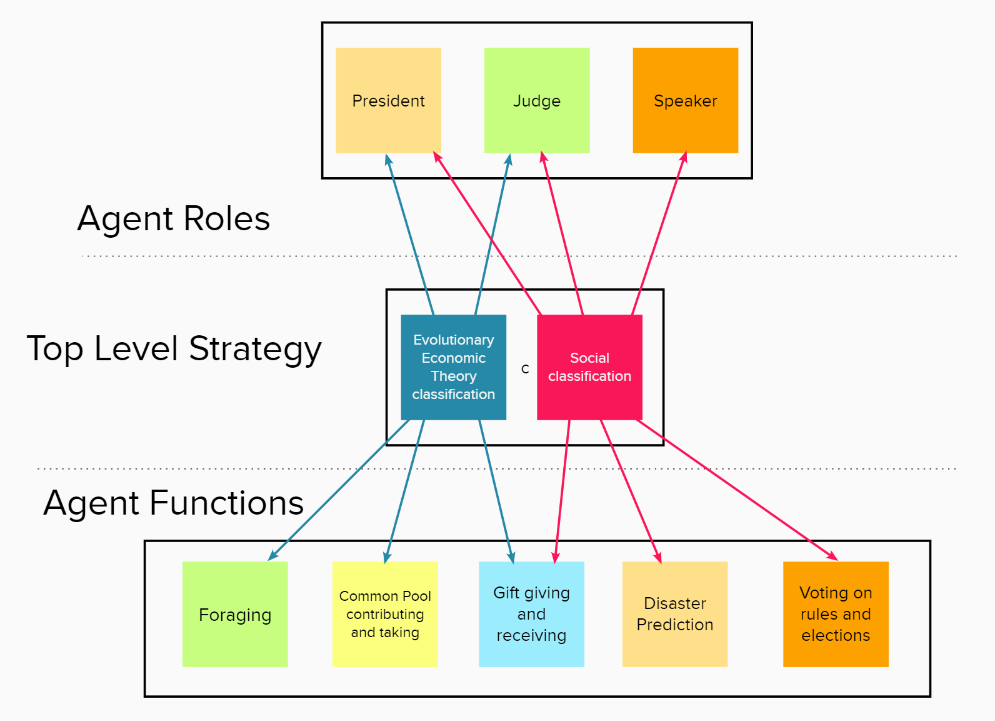
\includegraphics[width=0.49\textwidth]{10_team2_agentdesign/images/strategies.png}
        \label{fig: top level strategy}    
    }
    \subfigure[Ceremonial-Instrumental dichotomy]{
        \centering
        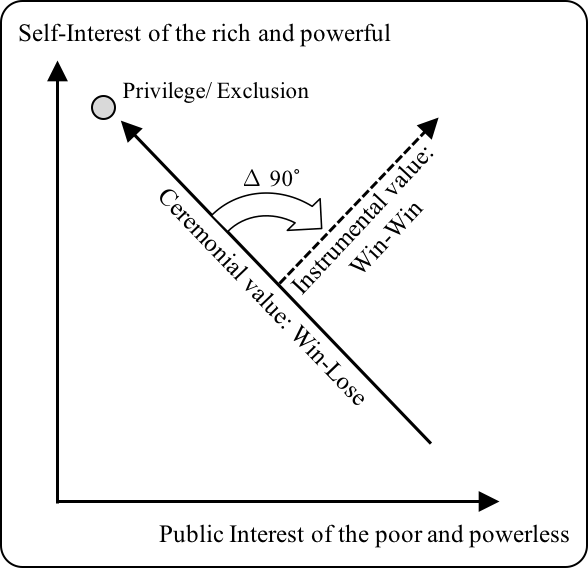
\includegraphics[width=0.49\textwidth]{10_team2_agentdesign/images/dichotomy.png}
        \label{fig: dichotomy}
    }
\end{figure}

\subsection{Evolutionary Economic Theory}
The term Evolutionary Economic Theory was first coined by economist Thorstein Veblen \footnote{https://www.cambridge.org/core/what-we-publish/elements/evolutionary-economics}. Evolutionary Economic Theory proposes that economic processes evolve, and it rejects the assumptions of classical rational choice theory. From Evolutionary Economic Theory, we categorised agent behaviour into distinct groups \footnote{https://www.cambridge.org/core/what-we-publish/elements/evolutionary-economics}. These groups are an altruist, fair sharer, and free rider. These are explained in Table~\ref{tab:Evolutionary Economic Theory Agent classifications}.


\begin{table}[!htb]
    \caption{Evolutionary Economic Theory Agent classifications}
    \label{tab:Evolutionary Economic Theory Agent classifications}
    \begin{tabular}{|c|m{0.3\textwidth}|p{0.4\textwidth}|}
    \hline
    \textbf{Agent classification} & \textbf{Definition}  & \textbf{Examples within the game} \\ \hline
    Altruist  & More concerned about the welfare of the group than themselves  & \begin{tabular}[p{0.4\textwidth}]{@{}p{0.4\textwidth}@{}}-Contributes a surplus to the common pool\\ -Generous with gifts\end{tabular}                                                     \\ \hline
    Fair Sharer                   & Contributes enough to the group  to negate their negative impact on it & \begin{tabular}[p{0.4\textwidth}]{@{}p{0.4\textwidth}@{}}-Contributes the minimum necessary amount of resources \\ -Gift allocation is measured and reasonable\end{tabular}                          \\ \hline
    Free rider                    & More concerned with their individual welfare than the welfare of the group & \begin{tabular}[p{0.4\textwidth}]{@{}p{0.4\textwidth}@{}}-Will not contribute enough to the common pool \\ -Gift requests above their requirement \\ -Will not give out gifts\end{tabular} \\ \hline
\end{tabular}
\end{table}
    

The advantage of using this theory over rational choice theory from classical economics is that it accounts for the irrational decisions agents or humans make when dealing with economic decisions, such as deciding how much to contribute to a common pool. Humans have evolved to develop heuristics \footnote{\url{https://www.sciencedirect.com/topics/social-sciences/heuristics}} which are "rules of thumb" in order to make economic decisions quickly and when all information is not present. These heuristics are typically based on emotion and will often result in irrational decisions; an example of this would be brand loyalty. This is very relevant within the context of the game because there is a cost to large computations (decision making). Also, there is an information failure \footnote{\url{https://www.economicsonline.co.uk/Market_failures/Information_failure.html}} as the agents often do not know the threshold of the common pool and other vital game metrics. This information failure forces agents to use heuristics similar to those used by real people. An excellent example of a heuristic within this agent strategy is the level of trustworthiness decided within the social dilemma. If every agent was rational and all information was present in the game, there is no need to trust or distrust agents as they would maximize both their welfare and that of others.

Another primary reason for selecting this theory as the basis of our design is to explore the ceremonial-instrumental dichotomy\footnote{\url{https://www.jstor.org/stable/3486187?seq=3\#metadata_info_tab_contents}}. This dichotomy is best represented by the graph in figure \ref{fig: dichotomy} and shows the importance of the game's setup. Our agent is attempting to oppose this traditional response to instrumental and ceremonial societies. It would be interesting to change the game's ceremonial and instrumental values by changing the setup. While the current game infrastructure does not support this, it would be interesting to investigate the ceremonial-instrumental dichotomy by allowing islands to invest resources into developing their foraging technology to obtain higher returns. It would be interesting to investigate how this instrumental shift would change our agent's strategy and others' actions. This update in technology would replace the ceremonial institutional set up of the IIGO as it becomes redundant. Allowing islands to invest in technological advancement would add an extra dimension to the game as it evolves, and the importance of the IIGO and other instrumental components would shift.

\subsection{Evolutionary Economic Theory Implementation}
%explain how we use the information from the theory

Figure~\ref{fig:methods-of-play} shows the different states of our agent's different methods of play. At any point during the game, the state of our agent is determined only by the level of the Common Pool. Our agent's objective is to oppose the strategies employed by other agents to attain stability in the game. To determine the method of play of the other agents, we look at whether the Common Pool is, on average, increasing or decreasing. If the pool is being depleted, it can be assumed that the other agents act as free-riders on average. To counteract this, we act as an altruist (see section \ref{sec:Common Pool Dilemma Strategy} for more detail). The average pool level is used because individual agent strategies are irrelevant for the game's overall course. Within the game, we also do not always have access to individual agents' contributions, which would be needed to classify them individually. This makes the average level of the Common Pool the only viable parameter. 

Our simulations demonstrated that starting the game in a "free-rider" state resulted in optimal agent performance and did not negatively impact the course of the game overall.

The default state for the agent is to be a "fair sharer." The agent will move into altruist mode when the weighted average of the Common Pool has dropped drastically. The agent considers a weighted average to ensure that the agent does not panic after every disaster and over contribute. The most recent turns will also be weighed higher to determine the course of the game. When the Common Pool stops decreasing, the agent will move back to fair sharer mode. Similarly, if the pool's weighted average increases by a large factor, then our agent moves into a free-rider state.

\begin{figure}
    \centering
    \subfigure[Method of Play diagram]{
    \centering
        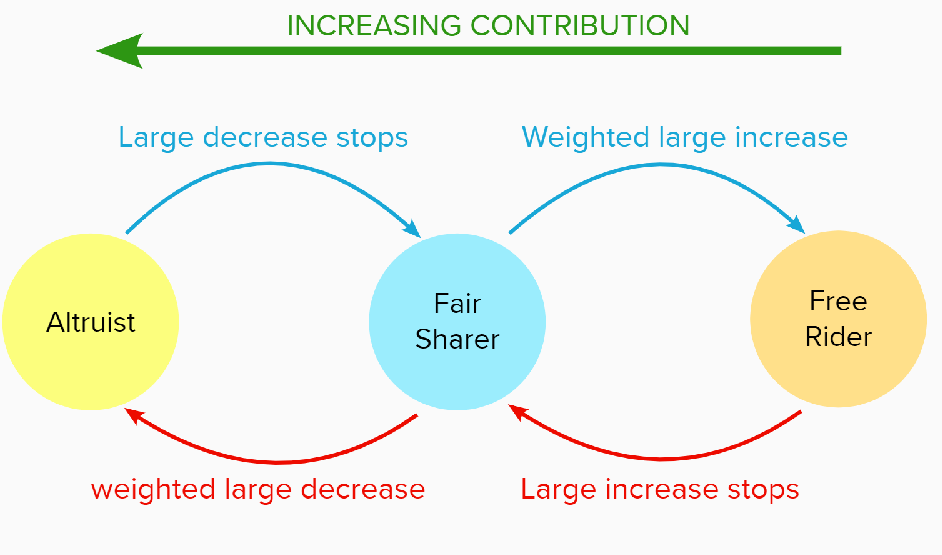
\includegraphics[width=0.49\textwidth]{10_team2_agentdesign/images/MethodofPlay.png}
        \label{fig:methods-of-play}
    }
    \subfigure[Social Classification Order]{
    \centering
    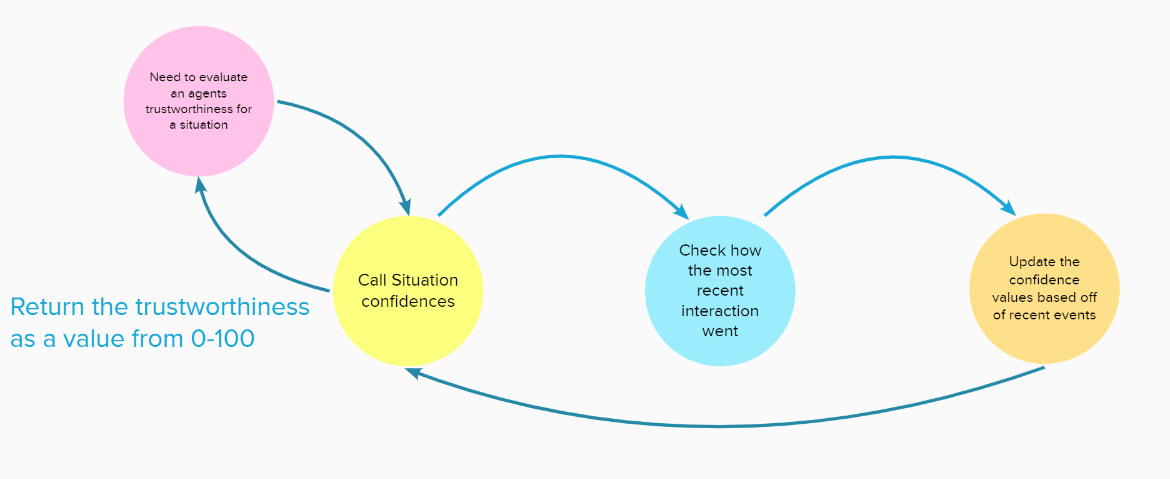
\includegraphics[width=0.49\textwidth]{10_team2_agentdesign/images/Social.png}
    \label{fig:social-order}
    }
\end{figure}



\subsection{Social Classification}
The agent forms an opinion on others depending on different situations. Initial testing suggested that another island's gift-giving behaviour does not necessarily correlate with their quality of predictions. Consequently, the trust of other agents is computed and stored separately for each situation. The agent uses the weighted average of past interactions with other agents to determine whether to trust them in each situation for future interactions. Using a weighted average to compute trust resulted in notably better agent performance. This is because the agent's trust in other agents considers all interactions with other agents while weighting recent interactions more heavily.

An integer value represents the agent's trust metric for each agent in each situation between 0 and 100, where 100 denotes full confidence and 0 a complete lack thereof. This value is used to compute the expected outcomes of situations. These are then compared with real events to update the agent's confidence in the other agents regarding this situation. For example, when the agent receives predictions from other islands, it computes the weighted average to check whether it trusts the island. Once a disaster occurs, the magnitude or timing of the disaster is compared with the other island's prediction. This reality is used to assess their behaviour and update the trust metric for that island relating to that situation. The list of different "situations" includes how an agent behaves in a role such as the President, Judge, Speaker, gift-giving, and disaster prediction. The overall structure of how the agent forms opinions on other islands is shown in Figure~\ref{fig:social-order}.

\section{Gift Giving and Receiving}
The agent must decide whether or not to respond to other agents' gift requests and how much to request from others through gifting. The implementation does not consider whether or not an agent is critical when requesting gifts and instead considers its current method of play and the trustworthiness of the requesting agent. Figure~\ref{fig: gifts} shows a decision tree for how the agent will allocate or request gifts, in which the agent splits up the gift request among the other agents to increase the likelihood of an agent allocating the gift.


\begin{figure}[!htb]
    \subfigure[Gift Giving and Receiving decision tree]{
        \centering
        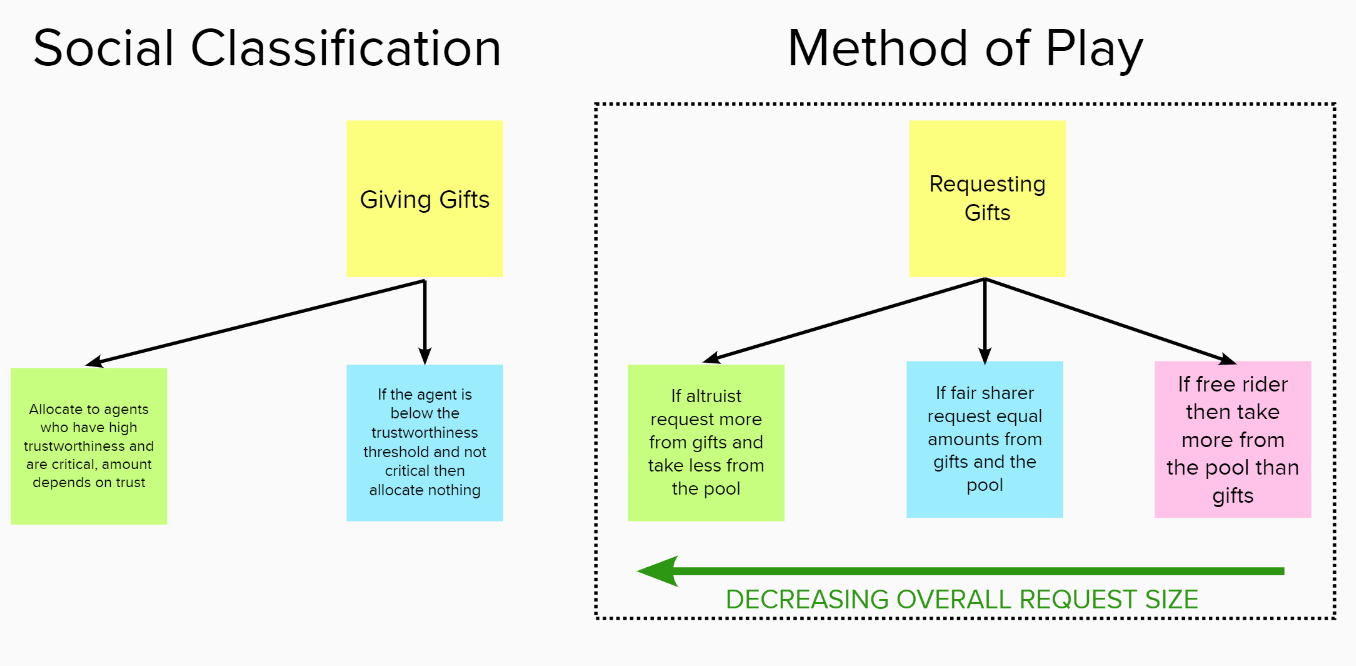
\includegraphics[width=0.49\textwidth]{10_team2_agentdesign/images/gifts.png}
        \label{fig: gifts}
    }
    \subfigure[Common Pool Strategy]{
        \centering
        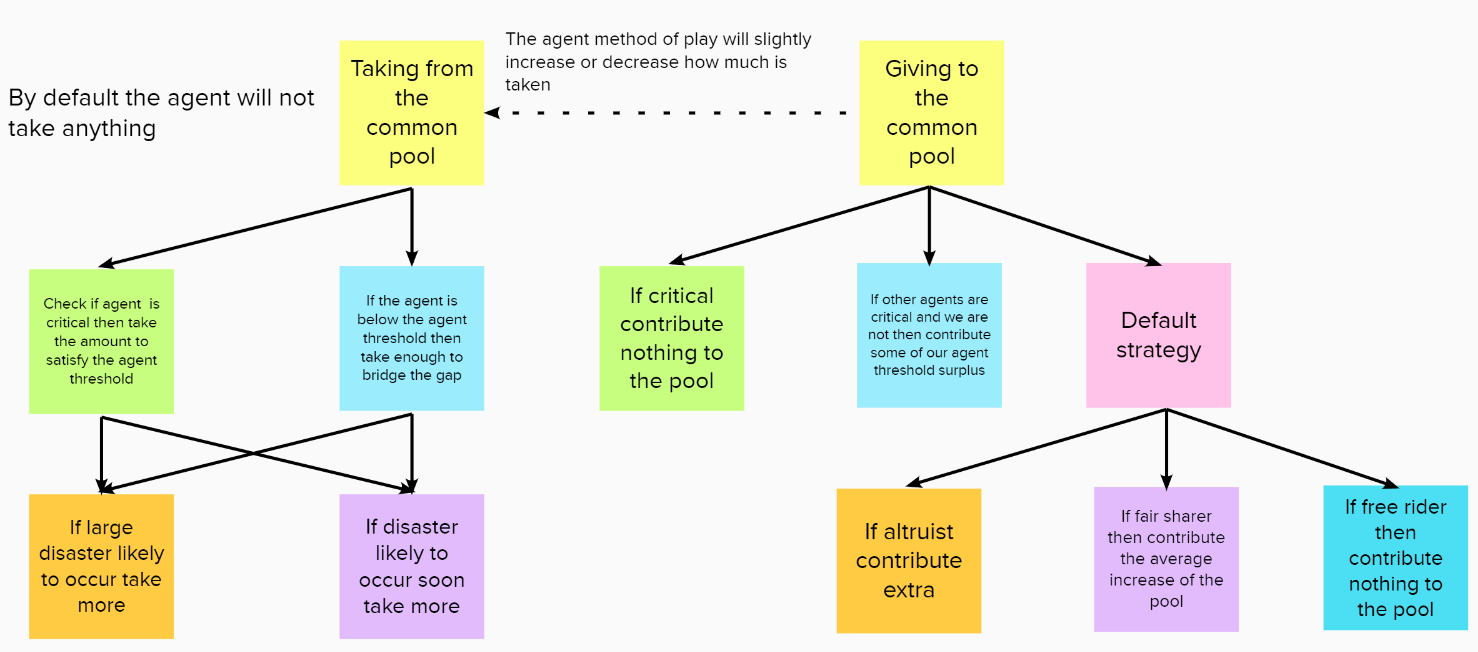
\includegraphics[width=0.49\textwidth]{10_team2_agentdesign/images/common_pool_strategy.png}
        \label{fig: common_pool_strategy}
    }
\end{figure}



Depending on the method of play, the agent will request more or fewer gifts. This is inversely proportional to the number of resources taken from the Common Pool. The agent obtains a larger proportion of its needed resources from gifting than the Common Pool in the altruist state. This is done to mitigate common pool depletion in the interest of the common good. In a Fair-Sharer state, the agent aims to obtain its resource target equally from gifts and the Common Pool. A minor surplus is also included in the resource target to ensure that the goal is met, given that gifts from other agents cannot be guaranteed. In a Free-Rider state, the agent takes the majority of its resources directly from the Common Pool but still requests gifts to build up its resources by taking advantage of relationships with other agents as well as a Common Pool surplus.

The \textbf{Gifts} social classification situation refers to both when an island requests a gift from our agent and when our agent requests a gift from that island. The balance between agent gift requests and responses is used as a basis for opinion formation on another agent. Other agents that fulfill the agent's requests are rewarded with higher trust. The agent's own gift requests tend to be small but are also proportional to its trust in each other agent. Every gift interaction is used to update the agent's trust in another island's gifting behaviour.

\section{Common Pool Dilemma Strategy} \label{sec:Common Pool Dilemma Strategy}
The Common Pool dilemma strategy can be split into two considerations. One consideration is the current method of play (altruist, fair sharer, and free-rider), and the other is the current game state. A decision tree showing the common pool strategy is shown in Figure~\ref{fig: common_pool_strategy}. These considerations decide whether and how much we contribute or take from the Common Pool.

\subsection{Method of play consideration} \label{ssec:Method of play consideration}
The primary consideration for giving to the Common Pool dilemma is the agent's current method of play. The agent's state is determined by the Common Pool level, as seen in Figure~\ref{fig:methods-of-play}. The agent's default state as a "fair sharer" contributes the average amount of other agents to the Common Pool. This is calculated by evaluating changes in the Common Pool level from the previous turn and averaging this quantity by dividing by the number of alive agents. If the Common Pool level decreases, the most recent Common pool increase is used to determine the amount given.

By using the average Common Pool contribution, the agent benefits from the forecasting of other agents. This benefit would arise should another agent have an advanced forecasting prediction that determines the Common Pool threshold and what is required to mitigate the effects of a disaster. In this case, the agent would then contribute a similar quantity of resources. This "herd-mentality" approach relies on the assumption that other agents make rational decisions. So if it is evident that other agents are acting irrationally, the agent deviates from this approach to an alternative state (to become either a free-rider or an altruist).

The agent is in an altruist state when the Common Pool is struggling, which often means that other agents act as free-riders. This is where the meta-strategy of Evolutionary Economic Theory comes into play. It is in the agent's interest to contribute much more to the Common Pool to alter the game's course in a positive direction and prevent the pool from being below the threshold when a disaster occurs. Therefore, the agent contributes more resources to enact this balance on the system. 
The altruist resource contribution is a larger factor of the weighted average contribution and can be tuned using the \emph{altruist factor} variable in the agent's configuration.

In a free-rider state, the Common Pool has a surplus, and the agent assumes other agents are on average operating as altruists. In this situation, the agent contributes less to the Common Pool and preserves resources to mitigate short and long-term risk. Contributing too much to the Common Pool no longer benefits the greater good, as these resources can still be used to forage and generate more resources. Therefore, the agent accumulates resources when others are too generous, allowing greater foraging investments and making it easier to help other agents if they struggle in the future.

The method of play also impacts how the agent decides to take from the Common Pool. After game state considerations are made, the agent adjusts how much it takes from the Common Pool according to its Agent State. Table~\ref{tab:Method of play common pool taking} outlines a summary of how the agent adjusts how much it takes and gives a justification for each action. The amount to take from the pool depends on how willing other agents are to contribute to the agent within the game's gift-giving section.  This means the agent must decide what proportion of the resource request must be taken from the Common Pool and from gifting, and this decision also factors in both common pool allocation as well as gift response predictions. When the agent is in a free-rider state, the common pool has a surplus, and so it makes more sense to take directly from the pool rather than requesting gifts. 

\begin{table}[!htb]
\centering
\caption{Method of play common pool taking}
\label{tab:Method of play common pool taking}
\begin{tabular}{|c|c|}
\hline
\textbf{Agent classification} & \textbf{How this impacts taking from the common pool}                              \\ \hline
Altruist                      & Pool is being depleted, best to not take from the pool                             \\ \hline
Fair Sharer                   & Gift requests and taking from the pool are equal                                   \\ \hline
Free rider                    & \multicolumn{1}{l|}{Pool has surplus, take from the pool rather than gift request} \\ \hline
\end{tabular}
\end{table}

\subsection{Game state consideration} \label{ssec:Game state consideration}
The primary consideration in taking from the Common Pool is the current game state. The key parameters (shown in Figure~\ref{fig: common_pool_strategy}) considered are whether the agent is critical and whether the agent has excess resources. This excess is calculated as the difference between the agent's current resources and the minimum resource threshold and the cost of living. Beyond this minimum resource level, the agent can survive one another turn. If the agent has fewer resources than these aggregated costs, the excess is zero. If there are excess resources, the agent will give some resources to the Common Pool. In this case, a strategic contribution is calculated. If the Common Pool threshold is known, the agent considers how many resources are required to attain this threshold. This is then spread over the expected number of turns until the next disaster is predicted to occur and the number of alive clients. If this is unknown, a default value is used to form an initial guess in the agent configuration. On top of this quantity, a strategic contribution is also calculated (see \ref{ssec:Method of play consideration}). The current method of play determines whether the disaster-determined contribution or the strategy-determined contribution is contributed to the pool. This amount is then contributed together with the current tax, unless there are no excess resources as this implies the agent is in a critical state and so all resources are preserved.

\section{Foraging Dilemma}
The foraging dilemma is split into two parts. One determines whether the agent should hunt or fish, and the other determines how many resources to spend on foraging. The foraging dilemma only depends on the current method of play. The method of play will impact the amount the agent uses to forages. If the Common Pool is doing well and the agent acts as a free rider, it will be more prone to take risk and contribute more to the foraging and vice versa. The decision to hunt or fish depends on the likely number of hunters in the next foraging event. The decision tree, Figure~\ref{fig: Hunt or fish decision tree }, shows how the agent decides whether to hunt or fish in a given turn. To determine the number of hunters in the next forage turn, the agent tracks how often each agent is a hunter and then sums up the probability of each agent hunting to find an overall number of likely hunters. The agent outputs a random number from 0 to 1, and if the number lies above the threshold, the agent will hunt. This threshold is determined by the number of likely hunters in the foraging. It implies there is an element of randomness to the agent's decision making, which will account for the unpredictability of dealing with other agents with their strategies.

\begin{figure}[!htb]
    \centering
    \subfigure[Hunt or fish decision tree]{
        \centering
        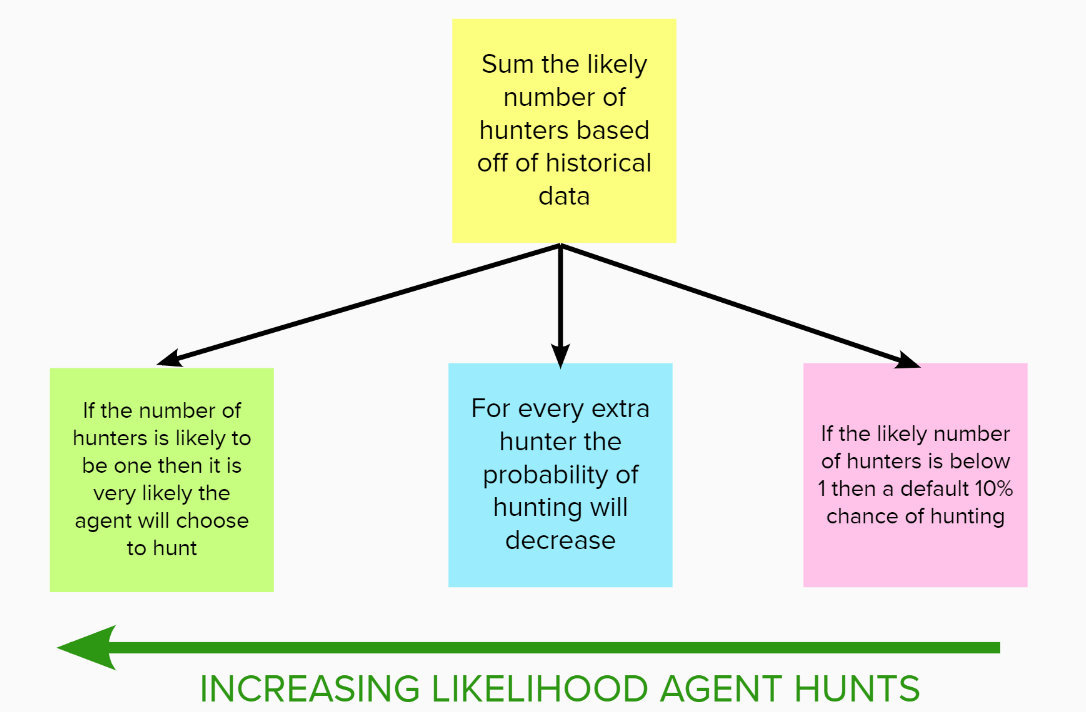
\includegraphics[width=0.49\textwidth]{10_team2_agentdesign/images/forage_decision.png}
        \label{fig: Hunt or fish decision tree }
    }
    \subfigure[Roles Decision Tree]{
        \centering
        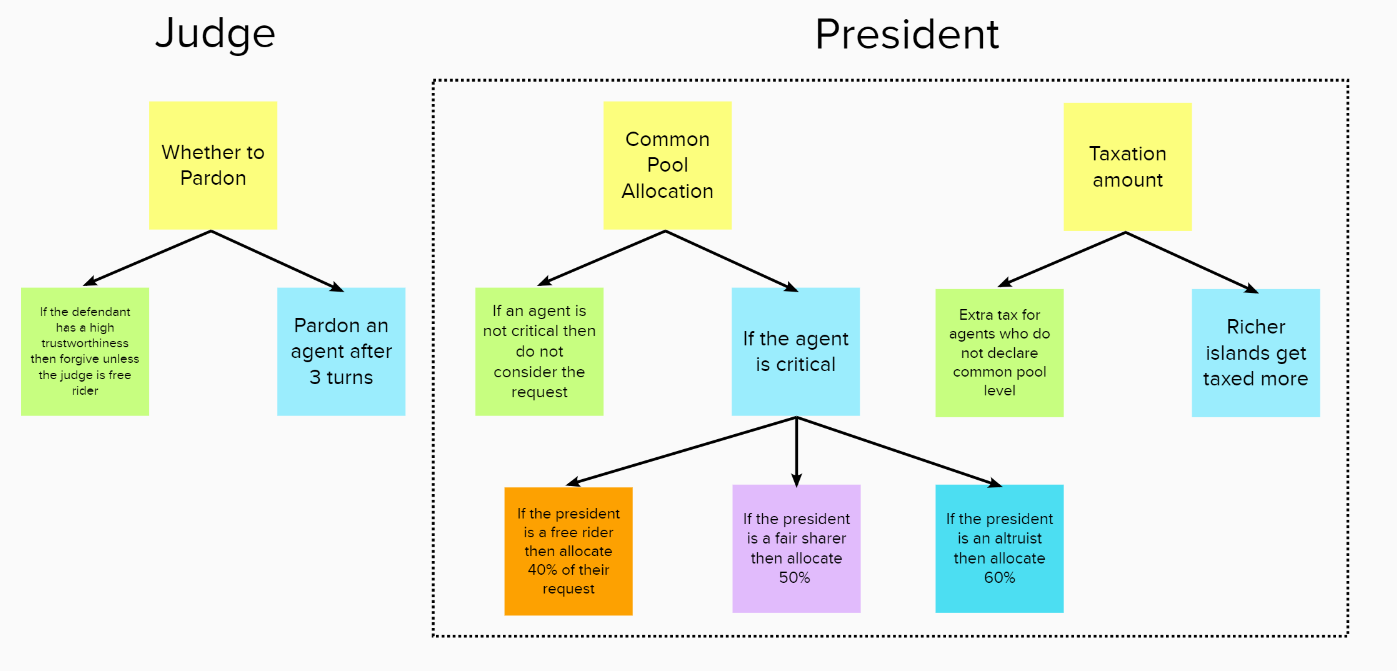
\includegraphics[width=0.49\textwidth]{10_team2_agentdesign/images/Roles Decision Tree.png}
        \label{fig: Roles Decision Tree}
    }
    \caption{Hunting or Fishing and Roles Decision Tree}
\end{figure}



The ideal distribution for foraging is to have two agents hunting and the remainder fishing. Hence, when the agent predicts one other agent will hunt, the agent is highly likely to choose to hunt too. The default threshold for hunting is 0.1, so the agent will hunt 10\% of the time when not considering the likely number of hunters. By assuming that any agent will hunt or fish with equal probability, the likelihood that there is one hunter is approximately 0.16. This implies hunting is an optimal strategy approximately 16\% of the time, so a threshold similar to this value is chosen. If the predicted number of hunters is above one, the following equation is used to determine threshold placement: $\text{Probability of agent hunting} = 0.95 - \text{Predicted number of hunters} \times 0.15$

The probability of choosing to hunt when the agent is confident only one other agent will also select hunt is 0.95. For each additionally predicted hunter, the probability will fall by 0.15. This 0.95 threshold is included in the agent configuration so it can be edited without changing the code. Hence, the foraging decision can be tuned. The agent checks if there are any excess resources after considering the minimum resource threshold not to be critical and the cost of living. If there are no excess resources, no resources are spent on foraging. If there is an excess of resources, a percentage of this excess is used on foraging. This percentage is controlled in the agent configuration. This approach ensures the agent has enough resources to survive another round, even in the worst case scenario when foraging returns are minimal.

\section{Role Strategies}

Figure~\ref{fig: Roles Decision Tree} shows a decision tree of how the agent acts under the two roles implemented. Due to time constraints, the base client implementation was used for the Speaker. The President is responsible for allocating resources from the Common Pool based on agent requests. The agent uses game state variables such as their critical status to determine if another agent is worthy of their resource request and the agent's allocation method based on the method of play is outlined in Table~\ref{tab:President allocation method of play}. When the agent is in a free-rider state, it is more selfish, while when it is an altruist, more of the others agents requests are approved. If an agent is not critical, it is highly unlikely that the agent will allocate them their requested resources as the purpose of the Common Pool should be to primarily mitigate the effects of disasters. Resources are allocated on a need-first basis, taxed proportionally to an agents resource level, and the strategy to determine taxation includes an additional penalty tax for agents who do not declare their resource levels. When evaluating another President's performance, the agent considers the percentage change in tax, the percentage of how much the agent is allocated with respect to how much it requests, and how much the agent takes with respect to how much the President allocates it.

\begin{table}[!htb]
\centering
\caption{President allocation method of play}
\label{tab:President allocation method of play}
\begin{tabular}{|c|c|}
\hline
\textbf{Agent classification} & \textbf{\% of request given} \\ \hline
Altruist                      & 60                           \\ \hline
Fair Sharer                   & 50                           \\ \hline
Free rider                    & 40                           \\ \hline
\end{tabular}
\end{table}

The agent implementation of the Judge evaluates whether an agent has broken any rules, as it should. However, to model real world corruption, the agent does not sanction agents that break rules if it considers them to be highly trustworthy (i.e., with a trust score above 80\%). The agents behaviour as a Judge is also determined by its state; when the agent is a free-rider, it sanctions fewer islands. The \textbf{Judge}'s situation, similar to the President, is used by the agent to determine what island to vote for as Judge. This is done by checking the past sanctions the agent received and their duration, to maxmimise personal benefit. The \textbf{RoleOpinion} social classification situation is used when the agent is the Judge and must decide whether or not to pardon other islands' sanctions, whom to choose as the next President whether or not an island has adhered by the rules. The Judge receives information for each island, such as the difference between how much an island contributed to the common pool and how much said they would. The agent uses these differences as a Judge to determine whether or not an island is trustworthy. During a role election, the agent checks its trust in the candidates for the appropriate situation, i.e., the situation when an agent is "President" for a future Presidential election. The agent will return a list of candidates in decreasing order of preference determined by the social classification. To do this, the agent sorts the candidates in terms of how much it trusts them.

\section{Disaster Prediction}
It is important for the agent to be capable of predicting both the severity and timing of disasters, in order to effectively make decisions for contributing to both the common pool and gifting resources to other agents.

Since the simulation is constructed through a series of successive turns, the occurrence of disasters throughout the game can be seen as a Binomial distribution: $D \sim \text{Bin}(n,p)$. In this equation, $D$ describes the number of disasters that occur, $n$ is the number of turns played and $p$ is the probability of a disaster occurring on a given turn.

The aim of our agent is to estimate the number of turns between disasters. We will denote this random variable as $T_D$, with our agent's aim being to find $E[T_D]$. To do this, our agent must estimate $p$. Therefore we have programmed our agent to find the Maximum Likelihood Estimator of $p$ for a Binomial RV\footnote{https://stats.stackexchange.com/questions/191444/variance-in-estimating-p-for-a-binomial-distribution}: $\hat{p} = \frac{D}{n} = \bar{X}$, where $\bar{X}$ is the sample mean of the RV $X$. The expectation of $T_D$ can be estimated using\footnote{https://math.stackexchange.com/questions/1299465/proof-variance-of-geometric-distribution}: $\hat{\mu}_{T_D}= \frac{1}{\hat{p}} = \frac{1}{\bar{X}}$. Thus, this is the optimal estimator for our agent to predict the number of turns between disasters. Furthermore, the confidence that our agent has in this prediction should be inversely proportional to the variance of $T_D$, i.e. how much does $T_D$ vary from the expected value we have found above? The expression for this variance is given below$^2$: $Var(T_D)= \frac{1-p}{p^2}$. 

However, given that our agent does not know the actual value of $p$ used in the simulation, our agent instead estimates the variance using: $\hat{\sigma}_{T_D}^2= \frac{1-\hat{p}}{\hat{p}^2}$. Now that an expression for the estimate of this variance has been obtained, two questions remain: ``what about the variance in $\hat{p}$" and ``how is this variance translated into a confidence value?" The variance of $\hat{p}$ is given by the following expression: $Var(\hat{p})= Var(\bar{X}) = \frac{Var(X)}{n}$. As previously, we do not know the exact value of $p$, making a calculation of $Var(X)$ impossible. However, we can make use of the fact that $Var(\hat{p}) \propto \frac{1}{n}$, by making our agents confidence in the prediction proportional to $n$ also. Secondly, the fact that variance can take values $\in [0,\infty]$ but confidence must take a value $\in [0, 100]$ makes mapping the values of variance that our agent calculates, to a confidence level, challenging. The solution our team opted for was to cap the max value of variance to some value $v_{cap_{T_D}}$, before translating this variance into a corresponding confidence value. This process is given by the equation below: $\text{confidence}_{T_D} = 100 - \frac{100 \cdot \text{min}(\frac{\hat{\sigma}_{T_D}^2}{kn}, v_{cap_{T_D}})}{v_{cap_{T_D}}}$ 
where $k$ is the tuning parameter for altering the dependence of the confidence on $n$. 

\subsection{Magnitude Prediction}
Our agent's strategy for predicting the magnitude of the next disaster shares many similarities with the strategy discussed in the last section. However, the magnitude of the next disaster is now distributed with an Exponential distribution: $M \sim Exp(\lambda)$. Once again, start by finding the MLE for the parameter $\lambda$ \footnote{https://en.wikipedia.org/wiki/Exponential\_distribution}: $\hat{\lambda} = \frac{1}{\bar{M}}$. Now we seek to estimate the expectation of $M$: $\hat{\mu}_M = \frac{1}{\hat{\lambda}} = \bar{M}$. Similarly, the variance of this RV is also useful to estimate $\hat{\sigma}_{M}^2= \frac{1}{\hat{\lambda}^2}$. As previously, there is also a variance in our estimation of $\hat{\lambda}$ that must be taken into account by making our confidence in this prediction proportional to $n$. Thus, the following expression should be used for calculating the confidence in the magnitude prediction: $\text{confidence}_M = 100 - \frac{100 \cdot \text{min}(\frac{\hat{\sigma}_{M}^2}{gn}, v_{cap_M})}{v_{cap_M}}$, where $g$ is the tuning parameter for altering the dependence of the confidence on $n$. 

\subsection{Overall Prediction}
The overall prediction that must be shared with teams during the IIFO session requires the following information: location, time until next disaster, magnitude and confidence. For our prediction of location, the middle of the archipelago is always given since the probability of a disaster occurring at a given location is uniform across the archipelago, meaning that there is no optimal prediction formula. Using the findings presented in the above sections, the formulas our agent will use to form a prediction about the next disaster are as follows:

\begin{align*}
    &x_{coord} = x_{min} + \frac{(x_{max}-x_{min})}{2}, y_{coord} = y_{min} + \frac{(y_{max}-y_{min})}{2}, \text{conf} =\frac{\text{conf}_{T_D} + \text{conf}_M}{2} \\
    &\hat{\mu}_{T_D}=\frac{1}{\bar{X}}, \hat{\mu}_M = \bar{M} \\
\end{align*}

\subsection{Combined Prediction}
Generating our own prediction is only the first part of the prediction making process. The second stage is to make use of other island's predictions during the IIFO session and using the social classification to decide prediction accuracy. When considering how much emphasis to put on a given island's prediction, we make use of two factors: 1.) Our island's confidence in each other island's prediction making. 2.) Each island's confidence in their own prediction, $P_i \in [0,100]$. These two considerations are then combined to create an overall confidence factor.

\section{Simulations}
Every function and agent consideration has tuneable parameter which can be edited without changing the whole agent. Figure~\ref{fig: Forage Untuned} shows how our agent reacts when it plays against itself and the foraging parameters are untuned. As you can see the game is unstable and the agents have a low survival rate. This is caused by an over contribution to the foraging dilemma, there is a point of marginal return with the foraging dilemma and spending too many resources can be wasteful. 

\begin{figure}[!htb]
    \centering
    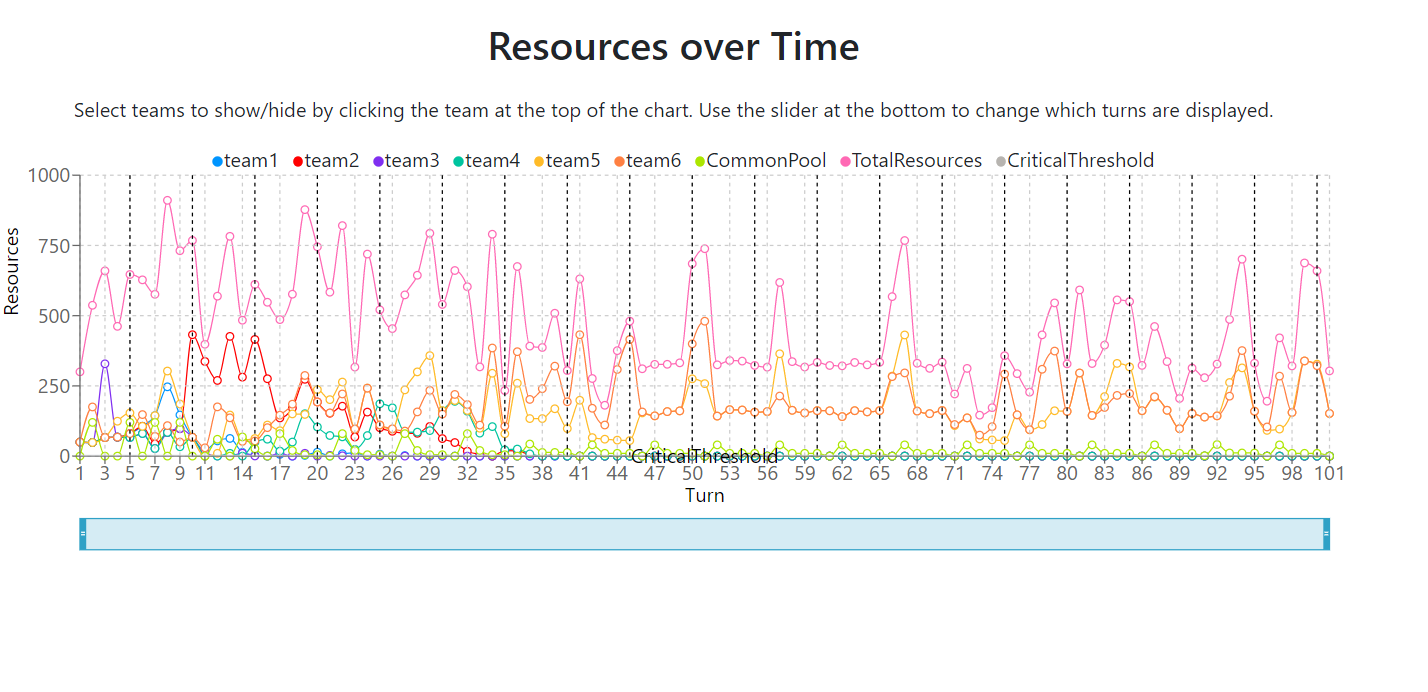
\includegraphics[width=0.6\textwidth]{10_team2_agentdesign/images/Forage Untuned.png}
    \caption{Untuned Forage Simulation}
    \label{fig: Forage Untuned}
\end{figure}

Figure~\ref{fig: Forage tuned} shows how our agents plays against itself when the foraging parameters are optimised. The amount of excess resources spent on foraging is more reasonable in this simulation, this results in a much higher survival rate and a more stable common pool.

\begin{figure}[!htb]
    \centering
    \includegraphics[width=0.6\textwidth]{10_team2_agentdesign/images/Forage tuned.png}
    \caption{Tuned Forage Simulation}
    \label{fig: Forage tuned}
\end{figure}

Figure~\ref{fig: altruist sim}  shows what happens when the agent plays itself and they are all altruists by default and do not move out of altruist. It can be seen that the agents over contribute to the Common Pool and are left with nothing to forage, this ends the game rather quickly. The simulation result was very similar for when all of the agents were free riders, the game would end in a couple of rounds after a lack of contribution to the common pool which caused impactful disasters.  This proves that being a free rider or altruist is not a rational decision and must be avoided. 

\begin{figure}[!htb]
    \centering
    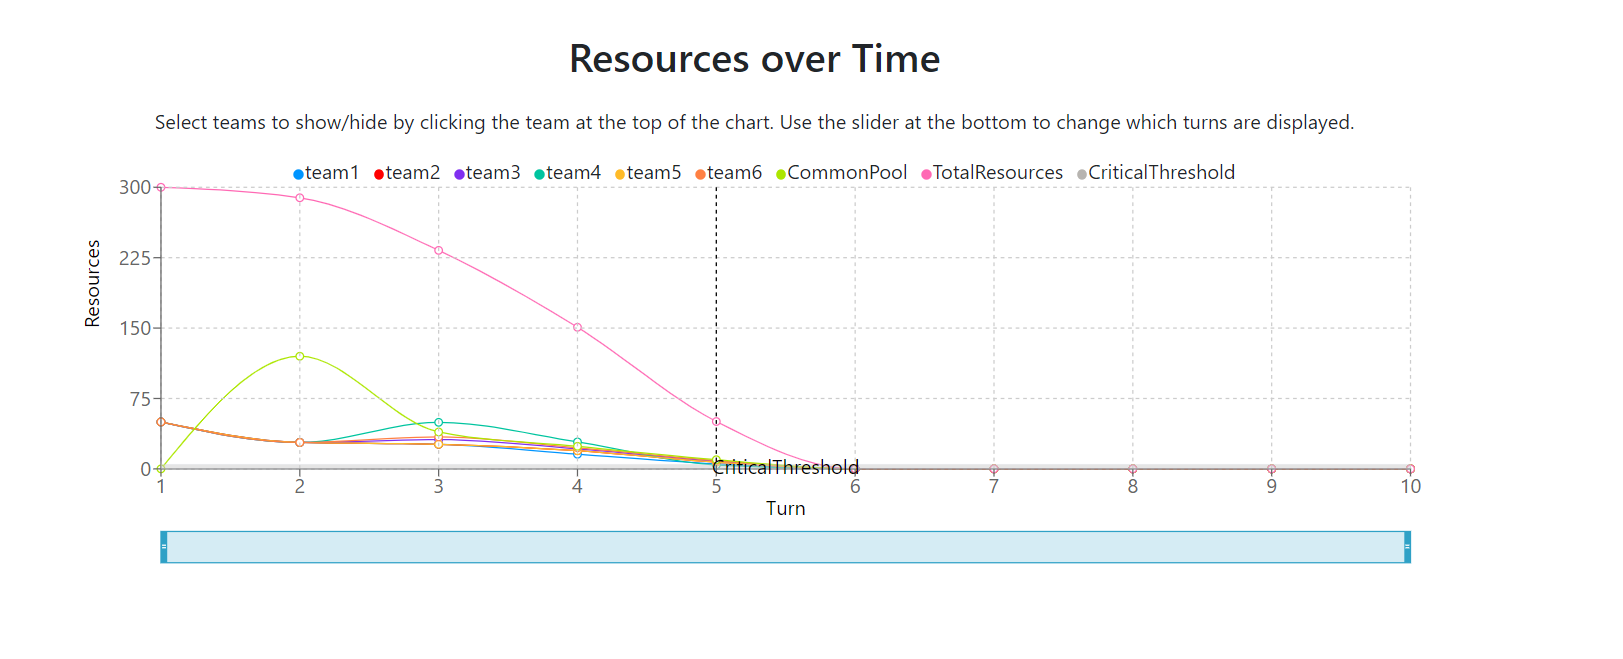
\includegraphics[width=0.7\textwidth]{10_team2_agentdesign/images/altruist sim.png}
    \caption{Altruist simulation}
    \label{fig:  altruist sim}
\end{figure} TODO: No image